\documentclass{article}

\usepackage{ctex}
\usepackage{cite}
\usepackage{bm}
\usepackage{setspace}
\usepackage{graphicx}
\usepackage{float}
\usepackage{stfloats}
\usepackage{placeins}
\usepackage{subfigure}
\usepackage{listings}
\usepackage{url}
\usepackage[linesnumbered,boxed,ruled,commentsnumbered]{algorithm2e}%%算法包,注意设置所需可选项
\usepackage{amsmath}
\newtheorem{definition}{定义}[section]
\newtheorem{theorem}{定理}[section]
\newtheorem{proof}{证明}[section]
\usepackage{setspace} 
\usepackage{diagbox}
\usepackage{multirow}
\usepackage[colorlinks,
linkcolor=blue,
anchorcolor=blue,
citecolor=blue]{hyperref}

\begin{document}
	\title{陈国良. 并行计算:结构·算法·编程[M]. 1999.}
	\author{屈彬}
	\maketitle
	
	\section{并行计算机系统及其结构模型}
		\subsection{并行计算(2019年7月2日)}
			\subsubsection{并行计算与计算科学}
				\begin{definition}[应用需求]
					应用需求分为三类,\textbf{计算密集}(Compute-Intensive)型应用,如大型科学工程计算与数值模拟;\textbf{数据密集}(Data-Intensive)型应用,如数字图书馆、数据仓库、数据挖掘和计算可视化等;\textbf{网络密集}(Network-Intensive)型应用,如协同工作、遥控和远程医疗诊断等。
				\end{definition}
				\begin{definition}[高性能计算和通信]
					High Performance Computing and Communication, HPCC。
				\end{definition}
				\begin{definition}[加速战略计算创新]
					Accelerated Strategic Computing Initiative, ASCI。
				\end{definition}
				\begin{definition}[美国能源部三大高性能计算实验室]
					Lawrence Livermore、Los Alamos、Sandia。
				\end{definition}
		\subsection{并行计算系统互连(2019年7月3日)}
			\subsubsection{系统互连}
				\begin{definition}[机群网络分类]
					\begin{enumerate}
						\item \textbf{系统域网络}:(System Area Network,SAN),连接短距离(3~25m)内的节点。
						\item \textbf{局域网络}:(Local Area Network,LAN),连接企事业单位内(500m~2km)内的节点。
						\item \textbf{节点内网络}:由\textbf{处理器总线}、\textbf{局部(本地)总线}、\textbf{存储器总线}构成。
						\item \textbf{小型机系统接口}:(Small Computer System Interface, SCSI)由\textbf{I/O总线}、\textbf{系统总线}构成。
					\end{enumerate}
				\end{definition}
				\begin{definition}[工作站机群]
					(Cluster of Workstations, COW),通过SAN/LAN互连的工作站组。
				\end{definition}
			\subsubsection{静态互连网络}
				\begin{definition}[对剖宽度]
					(Bisection Width):将网络划分为两等分所必须剪去的最少边数。
				\end{definition}
			\subsubsection{动态互连网络}
				\begin{definition}[总线分类]
					常用总线包括PCI、VME、Multibus、SBus、Microchannel和IEEE Futurebus。
				\end{definition}
				\begin{enumerate}
					\item \textbf{本地总线}:(Local Bus),CPU板级上的总线。
					\item \textbf{存储器总线}:存储器板级上的总线,主要指内存与CPU互连的总线。
					\item \textbf{数据总线}:I/O与通信板级上的总线,例如硬盘与内存之间的总线,以及网卡。
				\end{enumerate}
			\subsubsection{标准互连网络分类}
				\begin{enumerate}
					\item \textbf{光纤分布式数据接口}(Fiber Distributed Data Interface, FDDI),采用双向光纤令牌环提供100~200Mb/s的数据传输。
					\item \textbf{快速以太网}主流的互连网络,第三代以太网数据传输速度可达1Gb/s。
					\item \textbf{myrinet}由Myricom公司生产的千兆位包开关网。
					\item \textbf{高性能并行接口}(High Performance Parallel Interface, HiPPI),主要用于构筑异构计算机系统。
					\item \textbf{异步传输模式}(Asynchronous Transfer Mode, ATM),在光纤通信基础上建立起来的一种新的宽带综合业务数字网(B-ISDN)的交换技术。
					\item \textbf{无线带宽}(InfiniBand)。
				\end{enumerate}
		\subsection{并行计算机体系结构(2019年7月4日)}
			\subsubsection{并行计算机结构模型}
				大型并行机系统一般可分为六类机器:
				\begin{enumerate}
					\item \textbf{单指令多数据流}:(Single Instruction Multiple-Data, SIMD)。
					\item \textbf{并行向量处理机}:(Parallel Vector Processor, PVP)。
					\item \textbf{对称多处理机}:(Symmetric Multiprocessor, SMP)。
					\item \textbf{大规模并行处理机}:(Massively Parallel Processor, MPP)。
					\item \textbf{工作站机群}:(Cluster of Workstations, COW)。
					\item \textbf{分布共享存储多处理机}:(Distributed Shared Memory, DSM)。
				\end{enumerate}
				除SIMD外,其余五种皆为MIMD。
			\subsubsection{并行计算机访存模型}
				\begin{enumerate}
					\item \textbf{均匀存储访问}:(Uniform Memory Access, UMA),其特点包括:物理存储器被所有处理器均匀共享;所有处理器访问任何存储单元取相同的时间;每台处理器可带私有cache;外围设备也可以一定形式共享。这种系统由于高度共享资源又被称为\textbf{紧耦合系统}(Tightly Coupled System)。多核同构CPU系统的存储模型属于典型的UMA模型。
					\item \textbf{非均匀存储访问}:(Nonuniform Memory Access, NUMA)。
					\item \textbf{全高速缓存存储访问}:(Cache-Only Memory Access, COMA)。
					\item \textbf{高速缓存一致性非均匀存储访问}:(Coherent-Cache Nonuniform Memory Access, CC-NUMA)。
					\item \textbf{非远程存储访问}:(No-Remote Memory Access, NORMA)。
				\end{enumerate}
			\subsubsection{并行计算机存储组织}
				\begin{definition}[层次存储技术]
					利用程序局部性,设置多级存储系统。底层的存储器通常具有容量大、速度慢、成本低的特点,高层的存储器通常具有容量小、速度快、成本高的特点。层次存储技术出现的目的在于寻找性能与成本之间的平衡。
				\end{definition}
				\begin{definition}[高速缓存一致性问题]
					当处理器将新数据写入高层存储器时,需保证其他层次中存储器的数据对应的位置具有相同的副本。
				\end{definition}
	\section{当代并行计算机系统介绍}
	跳过第2章,它的内容与第1章存在大量重复。
	\section{并行计算性能评测}		
		\subsection{并行计算机的一些基本性能指标(2019年7月5日)}
			\subsubsection{CPU和存储器的某些基本性能指标}
				\begin{table}[H]
					\centering
					\begin{tabular}{|c|c|c|c|}
						\hline
						名称&符号&含意&单位\\
						\hline
						机器规模&$n$&处理器的数目&\\
						时钟速率&$f$&时钟周期长度的倒数&MHz\\
						工作负载&$W$&计算操作的数目&Mflop\\
						顺序执行时间&$T_{1}$&程序在单处理机上的运行时间&s(秒)\\
						并行执行时间&$T_{n}$&程序在并行机上的运行时间&s(秒)\\
						速度&$R_{n}=W/T_{n}$&每秒百万次浮点运算&Mflops\\
						加速&$S_{n}=T_{1}/T_{n}$&衡量并行机有多快&\\
						效率&$E_{n}=S_{n}/n$&衡量处理器的利用率&\\
						峰值速度&$R_{peak}=nR_{peak}^{'}$&所有处理器峰值速度之积&Mflops\\
						顺序峰值速度&$R_{peak}^{'}$&单个处理器的峰值速度&Mflops\\
						利用率&$U=R_{n}/R_{peak}$&可达速度与峰值速度之比&\\
						通信延迟&$t_{0}$&传送0-字节或单字的时间&$\mu$s\\
						渐进带宽&$r_{\inf}$&传送长消息的通信速率&MD/s\\
						\hline
					\end{tabular}
				\end{table}
			\subsubsection{通信开销测量方法}
				\begin{enumerate}
					\item \textbf{乒-乓方法}:(Ping-Pong Scheme)适用于一对节点之间通信开销的测量。
					\item \textbf{热土豆法}:(Hot-Potato),也称作\textbf{救火队法}(Fire-Brigade),适用于测量多个节点(两个以上)以环形方式通信,数据包传递一圈的通信开销。
				\end{enumerate}
				理论\textbf{点到点通信开销}$t(m)$是消息长度$m$(字节)的线性函数:
				$$t(m)=t_{0}+m/r_{\inf}$$
				其中$t_{0}$是通信启动时间($\mu$s),$r_{\inf}$是渐进带宽(MB/s)。
			\subsubsection{机器的成本、价格与性能/价格比}
				内容比较零碎,跳过。
		\subsection{加速比性能定律(2019年7月6日)}
			\subsubsection{Amdahl定律}
			\subsubsection{Gustafson定律}
			\subsubsection{Sun和Ni定律}
	\section{并行算法的设计基础}
		出于PAC比赛的需求,暂时先跳过第三章。
		\subsection{并行算法的基础知识}
		\subsection{并行计算模型(2019年7月7日)}
			并行计算模型是硬件和软件之间的一种桥梁(大雾,什么叫作``桥梁''),使用它能够设计分析算法,在其上高级语言能被有效地编译且能够用硬件实现。(我觉得作者没有把并行计算模型的用途讲清楚)
			\subsubsection{PRAM模型}
				即\textbf{并行随机存储机器}(Parallel Random Access Machine, PRAM),是一种抽象的并行计算同步模型。在这种模型中,假定存在着一个容量无限大的共享存储器;有多个同构处理器;在任何时刻各处理器均可通过共享存储单元相互交换数据以实现同步。根据对处理器读写时序的限制,又可分类为:
				\begin{enumerate}
					\item \textbf{不允许同时读和同时写}(Exclusive=Read and Exclusive-Write)的PRAM模型,记作\textbf{PRAM-EREW}。
					\item \textbf{允许同时读不允许同时写}(Concurrent-Read and Exclusive-Write)的PRAM模型,记作\textbf{PRAM-CREW}。
					\item \textbf{允许同时读和同时写}(Concurrent-Read and Concurrent-Write)的PRAM模型,记作\textbf{PRAM-CRCW}。
				\end{enumerate}
				不过,允许同时写显然是不现实的,所以对PRAM-CRCW模型做了进一步的约定:
				\begin{enumerate}
					\item \textbf{CPRAM-CRCW}:公共的PRAM-CRCW,只允许所有的处理器同时写相同的数。
					\item \textbf{PPRAM-CRCW}:优先的PRAM-CRCW,只允许最优先的处理器先写。
					\item \textbf{APRAM-CRCW}:任意的PRAM-CRCW,允许任意处理器自由写。
				\end{enumerate}
			\subsubsection{异步PRAM模型}
				记作APRAM,它的特点是\textbf{分相}(Phase),每个处理器都有其私有存储(书里称作``局存'')、私有时钟(书里称作``局部时钟'')和局部程序;处理器之间通过共享全局存储器进行通信;无全局时钟,各处理器异步地独立执行各自的指令;若处理器之间存在任何时序依赖关系(书中称作``时间依赖关系''),须通过插入同步路障(Synchronization Barrier)以保持依赖源和目标的执行顺序。
				
				APRAM模型具有四种访存指令:
				\begin{enumerate}
					\item \textbf{全局读}:将全局存储单元中的内容读入私有存储单元中。
					\item \textbf{局部操作}:对局存中的数执行操作,其结果是存入局存中。
					\item \textbf{全局写}:将局存单元中的内容写入全局存储单元中。
					\item \textbf{同步}:同步是计算中的一个逻辑点,在该点各处理器均需等待别的处理器到达后才能继续执行其局部程序。
				\end{enumerate}
			\subsubsection{BSP模型}
				整体同步计算模型(Bulk Synchronous Parallel),字面含义是``大''同步模型,该模型使用了三个属性描述:模块(Components)、选路器(Router)和同步路障器执行时间L(中文又称“超级步”)。BSP是一种MIMD-DM(DM:distributed memory)模型。
				
				在一个超级步中,每个处理器执行各自的局部计算,通过选路器接收和发送消息;然后作一全局检查(同步),以确定当前超级步是否已由所有的处理器完成;然后前进到下一个超级步。
				
				在分析BSP模型的性能时,假定局部操作可在一个超级步内完成。在每一超级步中,一个处理器至多发送或接收$h$条消息(称为\textbf{h-relation})。假定$s$是传输建立时间,$g$定义为每秒处理器所能完成的局部计算数目与每秒选路器所能传输的数据量之比,那么传送$h$条消息的时间开销为$gh+s$,若$gh\geq 2s$,则超级步步长$L\geq gh$(为什么?)。硬件可设置L的下限(例如宽的通信带宽减小$g$),而软件可设置L的上限(例如并行粒度越大,L越大)。
			\subsubsection{logP模型}
				\textbf{logP模型}是一种分布式存储的,点到点通信的多处理机模型,其中通信网络由一组参数来描述:
				\begin{enumerate}
					\item l(Latency)表示在网络中消息从源到目的地所遭到的\textbf{延迟}。
					\item o(Overhead)表示处理器发送或接收一条消息所需的\textbf{额外开销}。
					\item g(gap)表示处理器可连续进行消息发送或接收的最小时间间隔。
					\item P(Processor)表示处理器/存储器模块数。
				\end{enumerate}
		\section{并行算法的一般设计策略}
			\subsection{串行算法的直接并行化}
			
		\section{并行算法的基本设计技术}
			\subsection{划分设计技术}
				\subsubsection{均匀划分技术}
				\subsubsection{方根划分技术}
				
		\section{并行算法的一般设计过程}
		\section{基本通信操作}
		\section{稠密矩阵运算}
		\section{线性方程组的求解}
			\subsection{稀疏线性方程组求解}
				\subsubsection{共轭梯度法}
					(Conjugate Gradient),也叫\textbf{共轭斜量法}。其基本思想共轭梯度法用于求解类似于$\textbf{A}\textbf{x}=\textbf{b}$这样的一次方程组。通过对二次型函数
					$$f(\textbf{x})=\frac{1}{2}\textbf{x}^{T}\textbf{A}\textbf{x}-\textbf{b}^{T}\textbf{x}+c$$
					的变元$\textbf{x}$求导,得
					$$f^{'}(\textbf{x})=\textbf{A}\textbf{x}-\textbf{b}$$
					因此解方程组$\textbf{A}\textbf{x}=\textbf{b}$等价于求出当$f^{'}(\textbf{x})=\textbf{A}\textbf{x}-\textbf{b}=0$时对应的$\textbf{x}$(若$\textbf{A}$为实二次型,则$f^{'}(\textbf{x})=0$意味着$f(\textbf{x})$取得最小值)。
					
					要想充分理解共轭梯度法,我们首先要了解之前的用于求解大规模线性方程组的同类方法。
					
					\textbf{最速下降法(梯度下降法)}
					
					从任意一点$\textbf{x}_{(0)}$出发,每次都朝梯度方向(下降速度最快的方向)下降,从而得到解序列$\textbf{x}_{(1)}, \textbf{x}_{(2)},...$,直到两次下降的误差小于给定的误差上限。记第$i$次迭代的误差为$\textbf{e}_{(i)}=\textbf{x}_{(i)}-\textbf{x}_{(i-1)}$,残差为$\textbf{r}_{(i)}=\textbf{b}-\textbf{A}\textbf{x}_{(i)}$,其中$\textbf{x}$表示方程组$\textbf{A}\textbf{x}=\textbf{b}$的解。于是
					$$\textbf{r}_{(i)}=-f^{'}(\textbf{x}_{i})$$
					$$\textbf{x}_{(i+1)}=\textbf{x}_{(i)}+\textbf{a}_{(i)}\textbf{r}_{(i)}$$
					其中$\textbf{a}_{(i)}$为第$i$步沿着残差的方向$\textbf{r}_{(i)}$的步长。步长$\textbf{a}_{(i)}$选取的基本原则是尽量让下一次迭代中$f(\textbf{x}_{i+1})$的值更小,这样才能更快地到达$f(\textbf{x})$的全局最小值。把$f(\textbf{x}_{(i+1)})$看作是$\textbf{a}_{(i)}$的函数,要使得$f(\textbf{x})$最小,也就是求
					$$\frac{df(\textbf{x}_{(i+1)})}{d\textbf{a}_{(i)}}=0$$
					时的$\textbf{a}_{(i)}$值。根据链式法则,有
					$$\frac{df(\textbf{x}_{(i+1)})}{\textbf{a}_{(i)}}=\frac{df(\textbf{x}_{(i+1)})}{d\textbf{x}_{(i+1)}}\frac{d\textbf{x}_{(i+1)}}{d\textbf{a}_{(i)}}=f^{'}(\textbf{x}_{(i+1)})^{T}\frac{d\textbf{x}_{(i+1)}}{d\textbf{a}_{(i)}}=-\textbf{r}_{(i+1)}^{T}\textbf{r}_{(i)}$$
					当$\textbf{r}_{(i)}$与$\textbf{r}_{(i+1)}$正交时,$\textbf{r}_{(i+1)}^{T}\textbf{r}_{(i)}=0$,那么可以求出迭代步$\textbf{a}_{(i)}$
					$$\textbf{r}_{(i+1)}^{T}\textbf{r}_{(i)}=0$$
					$$(\textbf{b}-\textbf{A}\textbf{x}_{(i+1)})^{T}\textbf{r}_{(i)}=0$$
					$$(\textbf{b}-\textbf{A}(\textbf{x}_{(i)}+\textbf{a}_{(i)}\textbf{r}_{(i)}))^{T}\textbf{r}_{(i)}=0$$
					$$(\textbf{b}-\textbf{A}\textbf{x}_{(i)})^{T}\textbf{r}_{(i)}-\textbf{a}_{(i)}(\textbf{A}\textbf{r}_{(i)})^{T}\textbf{r}_{(i)}=0$$
					$$(\textbf{b}-\textbf{A}\textbf{x}_{(i)})^{T}=\textbf{a}_{(i)}(\textbf{A}\textbf{r}_{(i)})$$
					$$\textbf{a}_{(i)}=\frac{\textbf{r}^{T}_{(i)}\textbf{r}_{(i)}}{\textbf{r}^{T}_{(i)}\textbf{A}\textbf{r}_{(i)}}$$
					综合,最速下降法就是
					$$\textbf{r}_{(i)}=\textbf{b}-\textbf{A}\textbf{x}_{(i)}$$
					$$\textbf{a}_{(i)}=\frac{\textbf{r}^{T}_{(i)}\textbf{r}_{(i)}}{\textbf{r}^{T}_{(i)}\textbf{A}\textbf{r}_{(i)}}$$
					$$\textbf{x}_{(i+1)}=\textbf{x}_{(i)}+\textbf{a}_{(i)}\textbf{r}_{(i)}$$
					为了减小复杂度,也可以采用以下方法求$\textbf{r}_{(i+1)}$
					$$\textbf{b}-\textbf{A}\textbf{x}_{(i+1)}=\textbf{b}-\textbf{A}(\textbf{x}_{(i)}+\textbf{a}_{(i)}\textbf{r}_{(i)})$$
					$$\textbf{r}_{(i+1)}=\textbf{r}_{(i)}-\textbf{A}\textbf{a}_{(i)}\textbf{r}_{(i)}$$
					梯度下降法在迭代过程中迭代方向都与上一次迭代方向正交。
					
					\textbf{雅各比迭代法}
					
					学高数时似乎接触过。雅各比迭代要求线性方程组$\textbf{A}\textbf{x}=\textbf{b}$中的矩阵$\textbf{A}$为非奇异矩阵,对于一般矩阵$\textbf{A}$,我们可以把$\textbf{A}$拆分为矩阵$\textbf{D}$和$\textbf{E}$($\textbf{A}=\textbf{D}+\textbf{E}$),其中$\textbf{D}$是对角阵(可逆),$\textbf{E}$是剩下的部分,那么
					$$\textbf{A}\textbf{x}=\textbf{b}$$
					$$(\textbf{D}+\textbf{E})\textbf{x}=\textbf{b}$$
					$$\textbf{D}\textbf{x}=\textbf{b}-\textbf{E}\textbf{x}$$
					$$\textbf{x}=\textbf{D}^{-1}(\textbf{b}-\textbf{E}\textbf{x})$$
					为看得舒服,将$\textbf{x}=\textbf{D}^{-1}(\textbf{b}-\textbf{E}\textbf{x})$写作
					$$\textbf{x}_{(i+1)}=\textbf{B}\textbf{x}_{(i)}+\textbf{z}$$
					这就是雅各比迭代的迭代格式。其中$\textbf{B}=-\textbf{D}^{-1}\textbf{E}$,$\textbf{z}=\textbf{D}^{-1}\textbf{b}$。关于迭代格式的构造,知乎的答案\url{https://zhuanlan.zhihu.com/p/30965284}讲得很细。如果矩阵$\textbf{B}$的谱半径(最大特征值)小于1,那么迭代是可以收敛的,反之则不能收敛。
					
					梯度下降法与雅各比迭代法公共的主要缺陷是:为了收敛到解附近,迭代方向可能变了很多次,造成迭代次数增多,从而增加计算复杂度。
					
					\textbf{共轭梯度法}
					
					如果能够选取一系列线性无关的方向向量$\textbf{d}_{(0)},\textbf{d}_{(1)},\textbf{(d)}_{(2)},...,\textbf{d}_{(n-1)}$,沿着每个方向只迭代一次,最后就能到达解$\textbf{x}$处,迭代的次数最多为$n$次,可以解决梯度下降法和雅各比迭代法的问题。
					
					\textbf{共轭} 给定一个正定矩阵$\textbf{A}$,如果两个向量$\textbf{u}$和$\textbf{v}$满足$\textbf{u}^{T}\textbf{A}\textbf{v}=0$,则称$\textbf{u}$和$\textbf{v}$是关于矩阵$\textbf{A}$共轭的。
					
					现在我们来找一组关于线性方程组$\textbf{A}\textbf{x}=\textbf{b}$中矩阵$\textbf{A}$两两共轭的基向量$\textbf{d}$。问题在于如何寻找这样的$\textbf{d}$。
					
					我们先看一下残差向量$\textbf{r}$。对于第$i+1$次迭代中的残差$\textbf{r}_{(i+1)}$,根据最速下降法中的公式,有
					$$\textbf{r}_{(i+1)}=\textbf{b}-\textbf{A}\textbf{x}_{(i+1)}$$
					$$\textbf{r}_{(i)}=\textbf{b}-\textbf{A}\textbf{x}_{(i)}$$
					$$\textbf{x}_{(i+1)}=\textbf{x}_{(i)}+\textbf{a}_{(i)}\textbf{r}_{(i)}$$
					哎呀不管了,目前没找到有靠谱证明过程的资料,直接上共轭梯度法的公式吧
					$$\textbf{d}_{(0)}=\textbf{r}_{(0)}=\textbf{b}-\textbf{A}\textbf{x}_{0}$$
					$$\textbf{a}_{(i)}=-\frac{\textbf{d}^{T}_{(i)}\textbf{r}_{(i)}}{\textbf{d}^{T}_{(i)}\textbf{A}\textbf{d}_{(i)}}$$
					$$\textbf{x}_{(i+1)}=\textbf{x}_{(i)}+\textbf{a}_{(i)}\textbf{d}_{(i)}$$
					$$\textbf{r}_{(i+1)}=\textbf{r}_{(i)}-\textbf{a}_{(i)}\textbf{A}\textbf{d}_{(i)}$$
					$$\textbf{d}_{i+1}=\textbf{r}_{(i+1)}+\frac{\textbf{r}^{T}_{(i+1)}\textbf{r}_{(i+1)}}{\textbf{r}^{T}_{(i)}\textbf{r}_{(i)}}\textbf{d}_{(i)}$$
		\section{快速傅里叶变换}
		\section{并行程序设计基础}
		\section{共享存储系统并行编程}
		\section{分布存储系统并行编程}
			\subsection{基于消息传递的并行编程(2019年7月10日)}
				所谓基于消息传递的并行编程,是指用户必须显示地通过发送和接收消息来实现处理器之间的数据交换。根据问题分解的两种形式,消息传递并行性的开发也分为两种模式
				\begin{enumerate}
					\item \textbf{域分解}:将一个大的问题区域分解成若干个较小的问题区域,每个区域执行同样的指令,但处理的数据不同。通常采用SPMD(Single Process Multiple Data)编程模式实现。
					\item \textbf{函数分解}:又称\textbf{功能分解},将一个大问题分解成若干个子问题,每个子问题执行不同的指令。通常采用MPMD(Multiple Process Multiple Data)编程模式实现。
				\end{enumerate}
				\subsubsection{SPMD并行程序}
					SPMD按照节点的地位可分为两种结构
					\begin{enumerate}
						\item \textbf{主机/节点结构}:节点分为master和slave。
						\item \textbf{无主机结构}:每个节点都是对等的。
					\end{enumerate}
				\subsubsection{MPMD并行程序}
					实现子问题之间相互作用方式有两种
					\begin{enumerate}
						\item \textbf{数据流方式}:(Dataflow)根据子问题数据的相关性来组织并行,按\textbf{数据驱动}(Data-Driven)的方式决定并行执行的先后次序。
						\item \textbf{客户/服务器方式}:就是常见的C/S方式。
					\end{enumerate}
			\subsection{MPI并行编程(2019年7月10日)}
				(Message Passing Interface)。MPI进程是\textbf{重量级}、\textbf{单线程}的进程。
				\subsubsection{最基本的MPI}
					MPI标准包含6个基本函数
					\begin{table}[H]
						\centering
						\begin{tabular}{ll}
							\hline
							函数名 & 功能\\
							\hline
							MPI\_INIT & 启动MPI计算\\
							MPI\_FINALIZE & 结束MPI计算\\
							MPI\_COMM\_SIZE & 确定进程数\\
							MPI\_COMM\_RANK & 确定自己的进程标识符\\
							MPI\_SEND & 发送一条消息\\
							MPI\_RECV & 接受一条消息\\
							\hline
						\end{tabular}
					\end{table}
					下面以MPICH2为例说明个函数的详细信息。
					\\\textbf{MPI\_INIT(int *argc, char **argv)}\\
						启动MPI计算,argc、argv都是main函数的参数,将主函数参数传递给其他节点。
					\\\textbf{MPI\_FINALIZE()}\\
						结束MPI计算。
					\\\textbf{MPI\_COMM\_SIZE(comm, *size)}\\
						\begin{table}[H]
							\centering
							\begin{tabular}{lll}
								\hline
								输入输出类型 & 参数名 & 解释\\
								\hline
								IN & comm & 通信体(handle)\\
								OUT & size & 通信体comm中进程的个数(integer)\\
								\hline
							\end{tabular}
						\end{table}
					
					\textbf{MPI\_COMM\_RANK(comm, *pid)}\\
						\begin{table}[H]
							\centering
							\begin{tabular}{lll}
								\hline
								输入输出类型 & 参数名 & 解释\\
								\hline
								IN & comm & 通信体(handle)\\
								OUT & pid & 通信体comm中当前进程的标识符(integer)\\
								\hline
							\end{tabular}
						\end{table}
					\textbf{MPI\_SEND(*buf, count, datatype, dest, tag, comm)}\\
						\begin{table}[H]
							\centering
							\begin{tabular}{lll}
								\hline
								输入输出类型 & 参数名 & 解释\\
								\hline
								IN & buf & 待传输数据的内存首地址(可选参数)\\
								IN & count & 待传输数据的长度(integer)\\
								IN & datatype & 待传输数据的类型(handle)\\
								IN & dest & 目标进程的pid(integer)\\
								IN & tag & 消息标识符(integer)\\
								IN & comm & 通信体(handle)\\
								\hline
							\end{tabular}
						\end{table}
					\textbf{MPI\_RECV(*buf, count, datatype, source, tag, comm, status)}\\
					\begin{table}[H]
						\centering
						\begin{tabular}{lll}
							\hline
							输入输出类型 & 参数名 & 解释\\
							\hline
							OUT & buf & 数据存放位置的首地址(可选参数)\\
							IN & count & 数据的长度(integer)\\
							IN & datatype & 待传输数据的类型(handle)\\
							IN & source & 源进程的pid(integer)\\
							IN & tag & 消息标识符(integer)\\
							IN & comm & 通信体(handle)\\
							OUT & status & 状态对象(statuse)(这是什么?)\\
							\hline
						\end{tabular}
					\end{table}
					MPI数据类型与C语言数据类型对应关系如下
					\begin{table}
						\centering
						\begin{tabular}{ll}
							\hline
							MPI(C Binding) & C \\
							\hline
							MPI\_BYTE & \\
							MPI\_CHAR & signed char\\
							MPI\_DOUBLE & double\\
							MPI\_INT & int\\
							MPI\_LONG & long\\
							MPI\_LONG\_DOUBLE & long double\\
							MPI\_PACKED & \\
							MPI\_SHORT & short\\
							MPI\_UNSIGNED\_CHAR & unsigned char\\
							MPI\_UNSIGNED & unsigned int\\
							MPI\_UNSIGNED\_LONG & unsigned long\\
							MPI\_UNSIGNED\_SHORT & unsigned short\\
							\hline
						\end{tabular}
					\end{table}
				\subsubsection{一个基于MPICH实现多节点并行的例子}
					本节使用的例子详见``MPI\_demo/mat\_inc''目录。该程序的主要功能是给一片连续的内存中不同的位置赋不同的值。
					
					我有两台刀片服务器node02(内网地址192.168.1.101)、node03(内网地址192.168.1.103),采用粗粒度的域分解方式实现任务划分,两台机器分别处理内存的前半段和后半段。两台机器的MPI软件版本必须相同,我用的是MPICH3。基本的MPICH软件包只包含mpirun、mpiexec,用于执行MPI程序;编译采用MPI程序还需要安装MPICH-devel开发者软件包,包含mpicc编译器。两台刀片服务器的操作系统皆为CentOS(具体版本未知),互连方式为infiniteband。
					
					以下是步骤:
					\begin{enumerate}
						\item 首先确保node02与node03之间可以免密ssh登录。使用``ssh-keygen -t [rsa] [target host]''命令生成ssh-key,储存在id\_rsa、id\_rsa.pub文件中。
						\item 将用mpicc编译器编译好的程序分别拷贝到两个节点的同一相对目录下(mpirun命令会携带主节点的环境参数到从节点),注意代码中需要有根据进程号进行域分解的代码。
						\item 在主节点(我以node02为主节点)中通过``mpirun -np [主节点进程数] [可执行文件] : -host [从节点地址] -np [从节点进程数] [可执行文件]''执行程序。也可以通过machinelist添加更多的节点。
					\end{enumerate}
					
					以下是通过执行命令``mpirun -np 1 ./mat\_inc\_mpi.out : -host 192.168.1.103 -np 1 ./mat\_inc\_mpi.out''产的生输出结果,该结果与对应串行程序的输出相同,验证了并行程序的正确性。
					\begin{figure}[H]
						\centering
						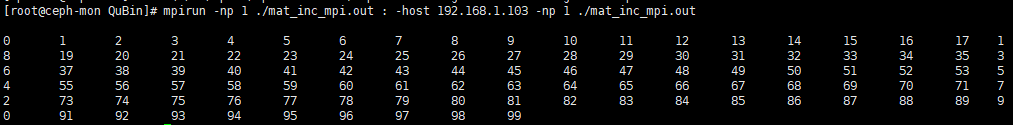
\includegraphics[width=1\linewidth]{image/mat_inc_mpi.png}
					\end{figure}
				\subsubsection{群体通信}
				
\end{document}